\documentclass[aspectratio=169]{beamer}

\mode<presentation> {
    \usetheme{Madrid}
    \usecolortheme{rose}
}

\usepackage{graphicx}
\usepackage{booktabs}
\usepackage{subfigure}
\usepackage[bookmarks=true]{hyperref}
\usepackage{blkarray}
\usefonttheme{serif}

\title[Scaling Laws]{
    Exploring Scaling Laws in LLM Pretraining
}

\author{Zibo Ren, Runlin Chen}
\institute[PKU]
{
    Peking University \\
    \medskip
    \texttt{\{2200010626,2200010848\}@stu.pku.edu.cn}
}
\date{\today}

\begin{document}

    \begin{frame}
        \titlepage
    \end{frame}

    \begin{frame}
        \frametitle{Overview}
        \tableofcontents
    \end{frame}


    \section{Scaling Laws}\label{sec:scalinglaws}

    \subsection{Chinchilla Scaling Law}\label{subsec:chinchilla}
    \begin{frame}
        \frametitle{Chinchilla Scaling Law}
        \begin{block}{Chinchilla Scaling Law}
            \begin{equation}
                \label{eq:chinchilla}
                \begin{aligned}
                    L(D, N) &= L_0 + A\cdot D^{-\alpha} + B\cdot N^{-\beta} \\
                \end{aligned}
            \end{equation}
        \end{block}
        \begin{itemize}
            \item $L(D, N)$ is the final validation loss.
            \item $D$ is the amount of data.
            \item $N$ is the number of parameters.
            \item $L_0$, $A$, $B$, $\alpha$ and $\beta$ are undetermined
            positive constants.
        \end{itemize}

        It only illustrates the loss at the end of training, but not the
        loss during training.
    \end{frame}

    \subsection{Scaling Law with LR Annealing (LRA)}\label{subsec:LRA}

    \begin{frame}
        \frametitle{Scaling Law with LR Annealing}
        \begin{block}{Scaling Low Formula}
            \begin{equation}
                \label{eq:scaling_low}
                \begin{aligned}
                    L(s) &= L_0 + A\cdot S_1^{-\alpha} - C\cdot S_2 \\
                    S_1 &= \sum_{i=1}^{s} \eta_i \\
                    S_2 &= \sum_{i=1}^{s} \sum_{k=1}^{i} (\eta_{k-1} -
                    \eta_k)\cdot\lambda^{i-k}
                \end{aligned}
            \end{equation}
        \end{block}

        \begin{enumerate}
            \item $L(s)$: the loss at step $s$.
            \item $\eta_i$: the learning rate at step $i$.
            \item $\lambda$: a hyper-parameter to notate the decay factor
            in LR annealing momentum.
        \end{enumerate}
    \end{frame}

    \begin{frame}
        \frametitle{Defect of Scaling Law with LR Annealing}
        \begin{enumerate}
            \item If the we add some iterations with learning rate 0 to
            the end of the training, according to
            (\ref{eq:scaling_low}), the loss will still decrease dual
            to $S_1$ is not change and $S_2$ is increasing.
            \item Multiplying the entire schedule elementwise by a positive constant larger than 1 always decreases the predicted loss.
            If we set the learning rate to approach positive infinity during the first iteration and subsequently fix it at zero, this would theoretically yield a negative loss value, which clearly contradicts empirical observations.
            \item The form of $S_2$ is based on observation, but it is lack of
            theoretical support.
        \end{enumerate}
    \end{frame}

    \subsection{Multi-Power Law}\label{subsec:MPL}

    \begin{frame}
        \frametitle{Multi-Power Law}
        \begin{block}{Multi-Power Law}
            \begin{equation}
                \label{eq:multi_power_law}
                \begin{aligned}
                    &L(t) = L_0 + A\cdot (S_1(t) + S_W)^{-\alpha} - LD(t)\\
                    &\text{where} \\
                    & LD(t) = B\sum_{k=1}^{t}(\eta_{k-1}-\eta_k)\cdot
                    G(\eta_k^{-\gamma}S_k(t)), \\
                    &S_k(t) = \sum_{i=k}^{t} \eta_i, \\
                    &G(x) = 1-(Cx+1)^{-\beta}
                \end{aligned}
            \end{equation}
        \end{block}

        \begin{enumerate}
            \item $A\cdot (S_1(t) + S_W)^{-\alpha}$ is an extension of
            Chinchilla scaling law.
            \item $LD(t)$ is a correction term to account for the
            learning rate decay.
            \item Actually $G(x)$ can be any increasing function that
            maps $[0, \inf]$ to $[0, 1]$.
        \end{enumerate}
    \end{frame}

    \begin{frame}
        \frametitle{Defect of Multi-Power Law}
        \begin{enumerate}
            \item If the we add some iterations with learning rate 0 between the schedule, the loss will not change actually.
            For example, the learning rate list [0.1,0,0.1,0] should get the same loss as [0.1,0.1].
            But using MPL, we will get different loss values because the $G(x)$ term cannot cancel each other.
            \item The theoretical support of MPL is deduced with the assumption that the learning rate schedule is SGD,
            which cannot demonstrate its validity in other circumstances.
        \end{enumerate}
    \end{frame}


    \section{Experiments}\label{sec:experiments}

    \begin{frame}
        \frametitle{Experiments Setup}
        \begin{enumerate}
            \item We use the loss curves of a 100M GPT model trained on
            20B tokens of data.
            \item We use 3 types of learning rate schedules: "8-1-1",
            warmup-stable-decay(WSD) and cosine.
            \item The total train step is 33907, we use the first 10000
            of one learning rate schedule to fit the parameters of
            the model and test the model on the full loss curve of
            the three learning rate schedules.
            \item For MPL, we conducted a set of ablation experiments.The following methods are all
            modified from the original MPL: OPL means $LD(t)=0$, LLDL means $G(x)=1$ and MEL means $G(x) = 1-e^{-Cx},\gamma = 0$
            \item Our code and data are available at \url{https://github.com/0Ishtar0/explore-scaling-law.git}
        \end{enumerate}
    \end{frame}

    \begin{frame}
        \frametitle{Experiments Results of LRA}
        We use cosine learning rate schedule to fit the parameters
        \begin{figure}
            \centering
            \subfigure[cosine learning rate]{
                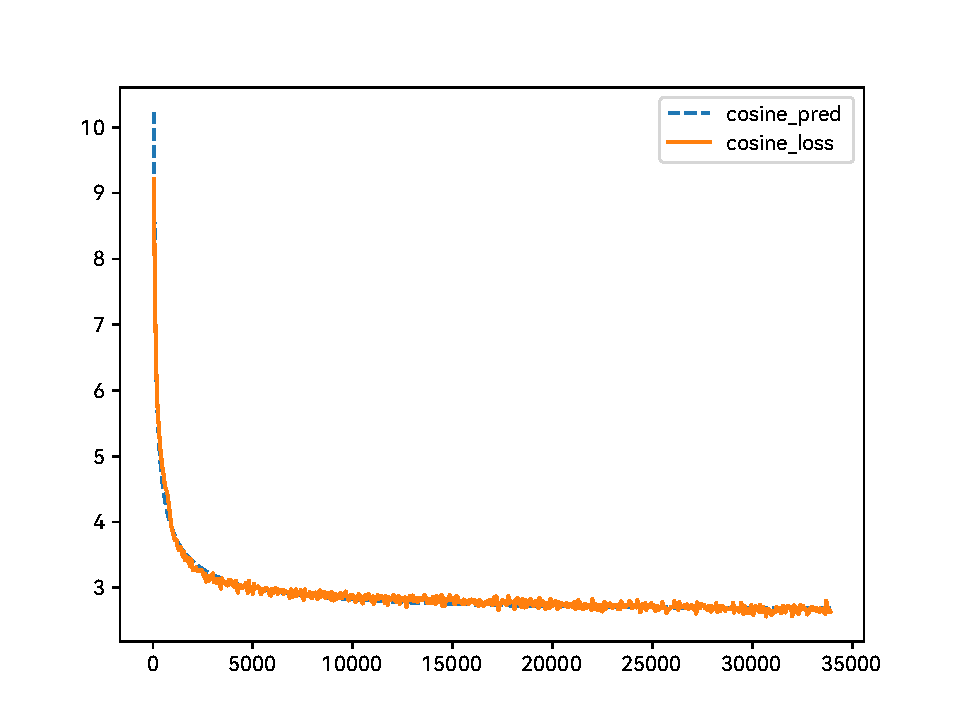
\includegraphics[width=0.3\textwidth]{fig/lra/cosine_fit.pdf}
            }
            \subfigure[8-1-1 learning rate]{
                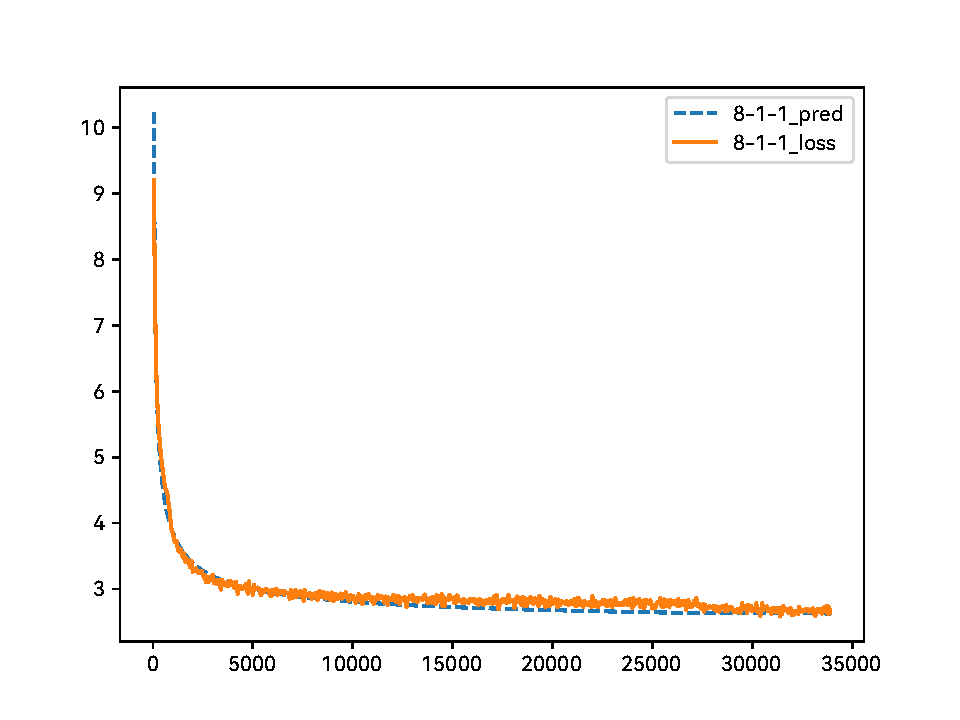
\includegraphics[width=0.3\textwidth]{fig/lra/8-1-1_fit.pdf}
            }
            \subfigure[WSD learning rate]{
                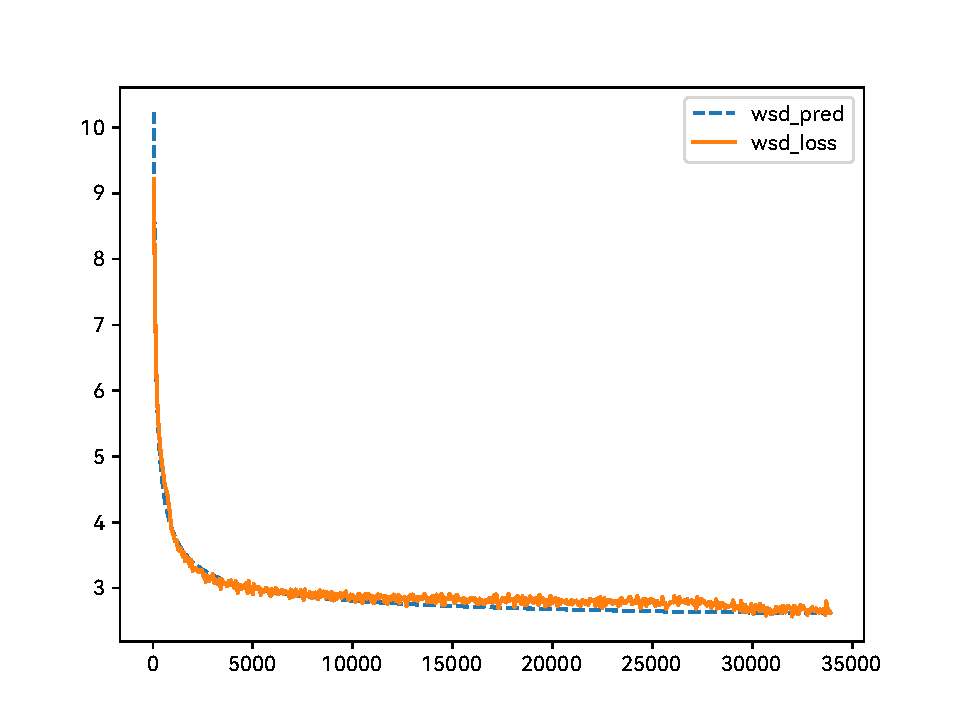
\includegraphics[width=0.3\textwidth]{fig/lra/wsd_fit.pdf}
            }\label{fig:figure}
        \end{figure}
    \end{frame}

    \begin{frame}
        \frametitle{Experiments Results of MPL}
        We use cosine learning rate schedule to fit the parameters
        \begin{figure}
            \centering
            \subfigure[cosine learning rate]{
                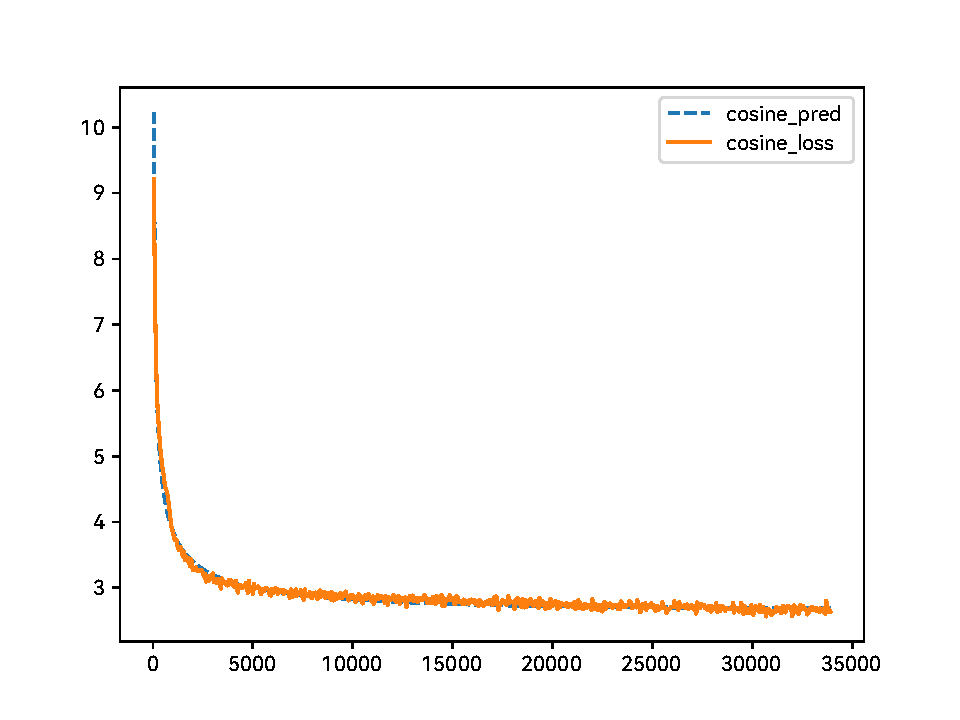
\includegraphics[width=0.3\textwidth]{fig/mpl/cosine_fit.pdf}
            }
            \subfigure[8-1-1 learning rate]{
                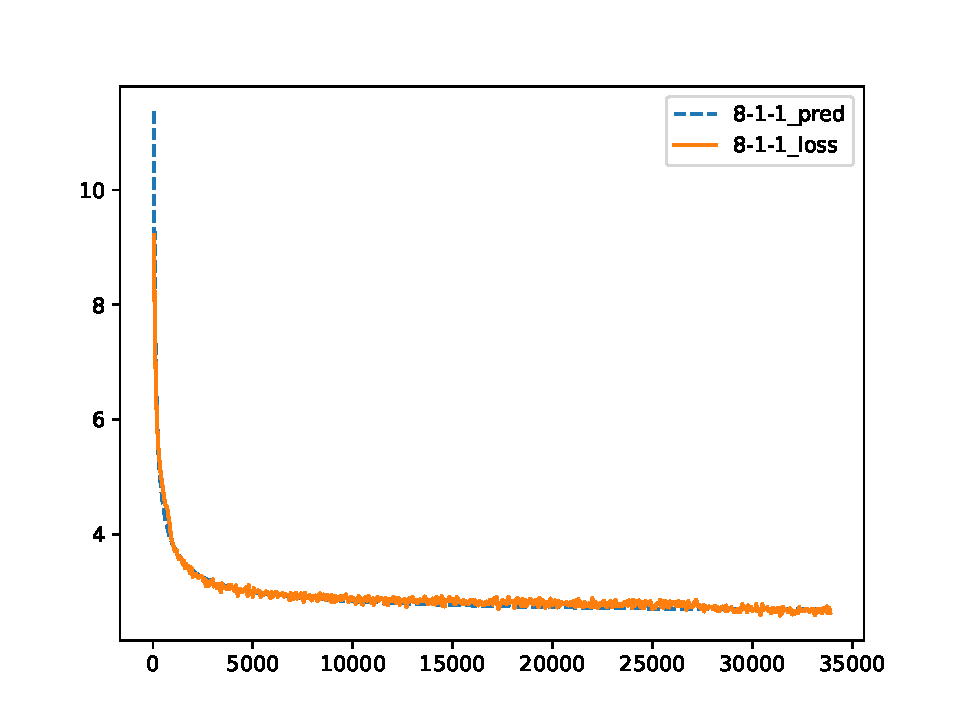
\includegraphics[width=0.3\textwidth]{fig/mpl/8-1-1_fit.pdf}
            }
            \subfigure[WSD learning rate]{
                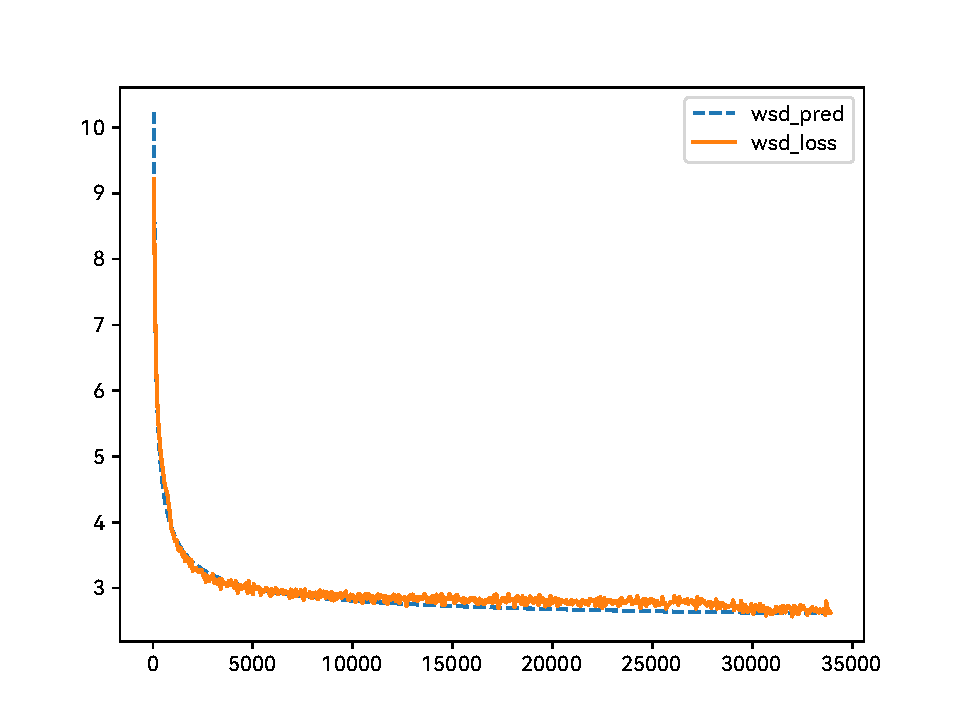
\includegraphics[width=0.3\textwidth]{fig/mpl/wsd_fit.pdf}
            }\label{fig:figure2}
        \end{figure}
    \end{frame}

    \begin{frame}
        \frametitle{Error of Fitting}

        The table below shows the fitting errors (MSE) of different scaling laws.
        \begin{table}[htbp]
            \centering
            \begin{tabular}{lcccc}
                \toprule
                Scaling Law & Schedule for Train & Cosine     & 8-1-1      & WSD        \\
                \midrule
                LRA         & Cosine             & 4.5861e-02 & 6.0476e-02 & 5.9120e-02 \\
                LRA         & 8-1-1              & 4.6447e-02 & 5.9456e-02 & 5.7880e-02 \\
                LRA         & WSD                & 4.4449e-02 & 5.4846e-02 & 5.3692e-02 \\
                MPL         & Cosine             & 4.6931e-02 & 8.8870e-02 & 8.9844e-02 \\
                MPL         & 8-1-1              & 4.5524e-02 & 7.8041e-02 & 7.6373e-02 \\
                MPL         & WSD                & 4.5555e-02 & 8.0023e-02 & 8.1387e-02 \\
                OPL         & Cosine             & 4.6876e-02 & 8.8801e-02 & 8.9809e-02 \\
                LLDL        & Cosine             & 4.6931e-02 & 8.8870e-02 & 8.9844e-02 \\
                MEL         & Cosine             & 4.6923e-02 & 8.9817e-02 & 8.8818e-02 \\
                \bottomrule
            \end{tabular}
            \caption{Fitting errors of different scaling laws}
            \label{tab:fitting_error}
        \end{table}


    \end{frame}

    \begin{frame}
        \frametitle{Phenomenon and Analysis}
        \begin{enumerate}
            \item[1] As shown in Table \ref{tab:fitting_error}, the fitting errors of all scaling laws under different training-test splits show minimal variation and remain below 0.1. This indicates that all scaling laws are effective in this set of experiments.
            \item[2] In the ablation experiments, we observe that modifications to the $LD(t)$ component result in negligible changes to fitting errors.
            This occurs because the learning rates in our experimental data vary smoothly, making this term several orders of magnitude smaller than the $S_1$ term, thereby exerting limited influence on the fitting outcomes.
        \end{enumerate}
    \end{frame}

    \begin{frame}
        \frametitle{Phenomenon and Analysis}
        \begin{enumerate}
            \item[3] Due to the minimal influence of the $LD(t)$ term, fitting curve of MPL closely approximates a simple power function.
            In contrast, fitting curve of LRA better captures the nuanced variations in loss (as illustrated in the figure below), thereby demonstrating superior fitting precision.
        \end{enumerate}
        \begin{figure}
            \centering

            \subfigure[LRA]{
                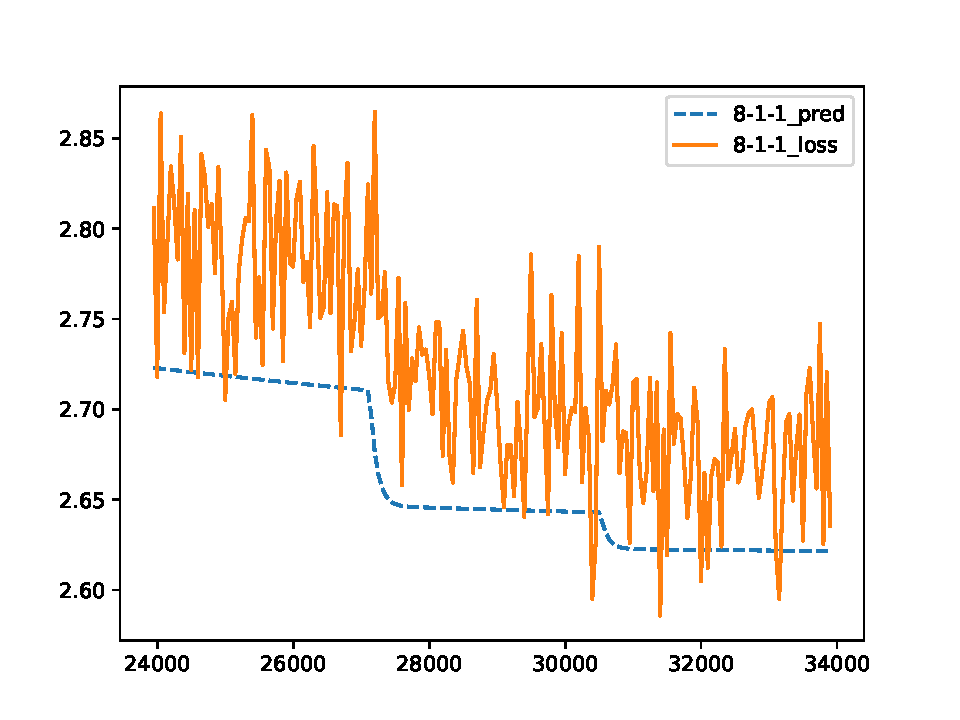
\includegraphics[width=0.4\textwidth]{fig/comparison/8-1-1_LRA}
            }
            \subfigure[MPL]{
                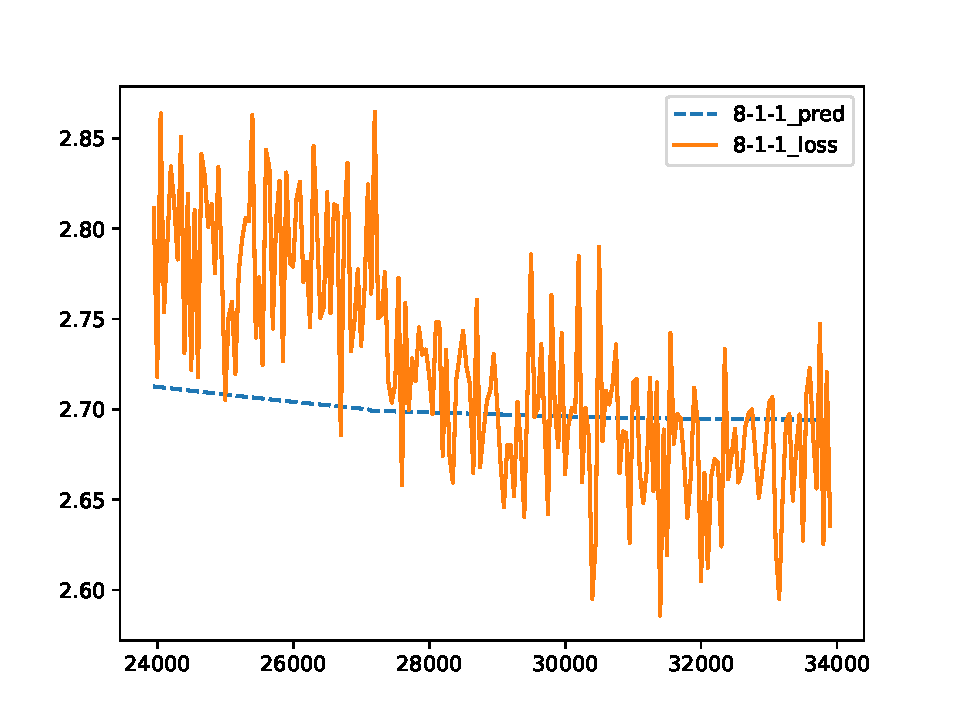
\includegraphics[width=0.4\textwidth]{fig/comparison/8-1-1_MPL}
            }
            \caption{Comparison of LRA and MPL fitting curves}\label{fig:figure3}
        \end{figure}
    \end{frame}

    % THANK FOR YOUR ATTENTION
    \begin{frame}
        \frametitle{}
        \begin{center}
            \Huge Thank You for Your Attention!
        \end{center}
    \end{frame}


\end{document}